% =============================================================================
% paper/nottingham_briefing.tex
% Research briefing for the Nottingham International Trade Summer School 2026
% Mentoring / office-hours session with A. Rodriguez-Clare and D. Donaldson.
% Self-contained: compile with pdflatex (or xelatex). Figures pulled from
% ../notebooks/_outputs/. References are a curated manual list (no bibtex needed).
% =============================================================================
\documentclass[11pt]{article}

\usepackage[a4paper,margin=2.5cm]{geometry}
\usepackage{amsmath,amssymb}
\usepackage{graphicx}
\usepackage{booktabs}
\usepackage{array}
\usepackage{caption}
\usepackage[table]{xcolor}
\usepackage{enumitem}
\usepackage{float}
\usepackage[T1]{fontenc}
\usepackage{lmodern}
\usepackage{mdframed}
\usepackage[colorlinks=true,allcolors=blue!55!black]{hyperref}

\graphicspath{{../notebooks/_outputs/}}

\captionsetup{font=small,labelfont=bf}
\setlist{itemsep=2pt,topsep=3pt}
\renewcommand{\arraystretch}{1.15}

\newcommand{\din}{d_{\mathrm{in}}}
\newcommand{\dout}{d_{\mathrm{out}}}
\newcommand{\sharecore}{\mathrm{Share\_core}}
\newcommand{\RCA}{\mathrm{RCA}}
\newcommand{\QB}{Q_B}

\newmdenv[linecolor=black!55,linewidth=0.6pt,backgroundcolor=black!3,
          roundcorner=3pt,skipabove=10pt,skipbelow=10pt,
          innertopmargin=9pt,innerbottommargin=9pt,
          innerleftmargin=10pt,innerrightmargin=10pt]{keybox}

% ---- title block ------------------------------------------------------------
\title{\vspace{-1.0cm}\textbf{\large Retrenchment or Reinvention?}\\[4pt]
\Large Firm-Level Capability Reconfiguration under Trade Shocks}

\author{%
\textbf{Giovanni Maran}\\[3pt]
\small Joint Doctoral Programme, University of Trento \& Free University of Bozen-Bolzano\\
\small\texttt{giovanni.maran@unitn.it}\\[6pt]
\small \emph{Supervisors:} Chiara Tomasi \& Stefano Schiavo (University of Trento)}

\date{}

\begin{document}
\maketitle
\thispagestyle{empty}

\begin{keybox}
\noindent\textbf{The project in one paragraph.}\ When a trade shock degrades the value
of a firm's existing activities, does the firm \emph{retrench} toward a coherent
capability core, or \emph{reinvent} itself by exploring new capability bundles? I
measure the firm's export basket as a position in a firm--product \emph{capability
network}, split diversification into an \emph{in-block} margin $\din$ (deepening the
core) and an \emph{out-of-block} margin $\dout$ (exploring beyond it), and ask how a
predetermined, continuous tariff shock moves the two. The static capability map is
already built on Chinese customs microdata (\S\ref{sec:china}); the causal panel is the
next step (\S\ref{sec:panel}). I would value your view on the mechanism, on the
identification, and on whether a tractable model can rationalise the sign
(\S\ref{sec:questions}).
\end{keybox}

\vspace{2pt}
{\small\tableofcontents}
\bigskip

% =============================================================================
\section{The question and why it is open}
\label{sec:question}
% =============================================================================

The empirical trade literature has measured, in great detail, how tariff shocks move
firm \emph{performance}: productivity, markups, employment, survival
(Pavcnik 2002; Topalova 2010; Amiti--Konings 2007; Le \& Tomasi 2023). It is almost
silent on what those shocks do to the \emph{composition} of the firm's activity --- which
products are kept, dropped, or newly entered, and whether the surviving basket is a
\emph{deepening} of a related core or a \emph{scattering} into new domains. This is the
object I want to make causal.

The reason the sign is genuinely open is theoretical. March's (1991)
exploitation--exploration tension says a firm whose core is threatened can either
intensify what it knows (retrench) or search outward (explore), and his own result is
that organisations systematically \emph{over-exploit}. Several literatures sharpen this
into a directional prediction:

\begin{itemize}
  \item \textbf{Retrenchment (H1, the modal prior).} Sunk-cost and re-entry-cost
        hysteresis (Crozet et al.\ 2021), variance-minimisation through within-cluster
        deepening (Bottazzi--Secchi 2006; Vannoorenberghe 2016; Crozet et al.\ 2025),
        and the competition-to-coherence evidence of Valvano--Vannoni (2003) and the
        product-vector consolidation of Fontagn\'e et al.\ (2018) all point to
        $\din\!\uparrow$, $\dout\!\downarrow$, $\sharecore\!\uparrow$.
  \item \textbf{Reinvention (H1$'$, the frontier-firm tail).} Penrose (1959),
        Teece (1982), the moderate-shock search models of Matsusaka (2001) and
        Bernardo--Chowdhry (2002), and escape-competition (Aghion et al.\ 2005;
        Akcigit--Melitz 2022) leave open $\dout\!\uparrow$ for firms with slack and a
        defensible core.
\end{itemize}

\noindent The economic-complexity toolkit (Hidalgo--Hausmann 2009; Tacchella et al.\
2012; Pugliese et al.\ 2019; Bruno et al.\ 2023; De Stefano et al.\ 2025) gives me the
\emph{measurement instrument} for capability structure --- a block-modular firm--product
partition --- but it has been used almost exclusively descriptively. The strategic-%
dependency literature (Farrell--Newman 2019; Arjona et al.\ 2023; Korniyenko et al.\
2017) identifies \emph{which} products carry geopolitical leverage but has no firm-level
causal test. The contribution I am aiming for sits in the empty intersection:
\emph{a causal estimate of the direction of capability adjustment to a predetermined
trade shock, with the strategic-dependence content of the product as the key moderator.}

% =============================================================================
\section{Preliminary evidence: the capability map of Chinese exporters}
\label{sec:china}
% =============================================================================

Before any causal claim, the measurement layer has to be real and economically legible.
I build it on Chinese firm$\times$product$\times$destination$\times$year customs exports.
For the 2008--2015 window the firm--product--year panel has $11.9$M rows over $372{,}030$
firms and $4{,}657$ HS6 products. To work with an established-exporter core I keep firms
that export in \emph{every} year of the window: $71{,}017$ firms --- only $19\%$ of the
count, but $62\%$ of export value. The export basket is binarised with the firm-level
Balassa index ($\RCA_{fp}>1$), giving a bipartite incidence with $\sim$1.1M links. Both
firm diversification and product ubiquity are heavily right-skewed (Fig.~\ref{fig:dist}
in the appendix), the usual complexity signature.

\begin{keybox}
\textbf{How the capability blocks are found (the algorithm, in plain terms).}\ The
firm--product matrix is a \emph{bipartite} graph: firms on one side, products on the
other, an edge whenever a firm has $\RCA>1$ in a product. A ``capability block'' is a
set of firms \emph{and} products that link among themselves far more densely than chance
would predict. ``Than chance'' is made precise by a null model. Bipartite modularity
$\QB$ (Barber 2007) scores a partition by the within-block edges \emph{in excess} of those
expected if every firm and every product kept its own number of links but rewired at
random --- the expected edge between firm $f$ and product $p$ is $k_f d_p/m$
(degree$\times$degree over total links). BRIM is the heuristic that maximises $\QB$. The
\emph{bipartite} null is the whole point: off-the-shelf optimisers (Louvain, Leiden) use
a \emph{one-mode} null that ``expects'' firm--firm and product--product edges which cannot
exist in a bipartite graph; that mis-specified baseline inflates apparent within-block
density and \emph{over-segments} (here $13$ and $9$ blocks against BRIM's $5$). A
resolution parameter $\gamma$ scales the null ``charge'' for grouping two nodes: $\gamma=1$
is standard modularity, $\gamma>1$ charges more and returns more, smaller blocks. I use
BRIM at $\gamma=1$ as the baseline and report $\gamma=2$ below.
\end{keybox}

\paragraph{Capability blocks are real, and they are not HS sectors.} Maximising Barber's
(2007) bipartite modularity (BRIM) on the incidence matrix yields \textbf{five capability
blocks} with a strong modular signal, $\QB=0.505$. The blocks have a clear economic
identity (Table~\ref{tab:blocks}, Fig.~\ref{fig:blocksec}): a large machinery and
electrical \emph{generalist} block (51\% of firms, the assembly base), a paper/light-%
manufacturing block (23\%), a near-pure \emph{textiles} block (15\%), a chemicals-plus-%
agri-food block (11\%), and a tiny ultra-specialised diamond satellite. The data-driven
partition is \emph{not} a relabelling of HS sectors: against the HS-section
partition it scores $\mathrm{ARI}=0.29$, $\mathrm{NMI}=0.43$, with blocks spanning on
average thirteen HS sections. The block is a capability object, not an industry code ---
which is exactly what makes the $\din/\dout$ split meaningful.

\begin{table}[H]\centering\small
\caption{The five capability blocks (2008--2015, HS6; $71{,}017$ established exporters).}
\label{tab:blocks}
\begin{tabular}{@{}clp{7.0cm}@{}}
\toprule
Block & Firms & Dominant content \\
\midrule
B0 & 36{,}321 (51\%) & Machinery \& electrical 36\%, base metals 24\%, instruments 7\% --- the large \emph{generalist} block \\
B2 & 16{,}095 (23\%) & Paper 16\%, misc.\ manufacturing, packaging --- light manufacturing \\
B1 & 10{,}870 (15\%) & \textbf{Textiles 95\%} --- apparel, cotton, man-made fibres (pure) \\
B3 &  7{,}691 (11\%) & \textbf{Chemicals 48\% + agri-food $\sim$41\%} (vegetables, foodstuffs, animals) \\
B4 &     40 (0\%)    & Precious 100\% --- diamonds (pure satellite) \\
\bottomrule
\end{tabular}
\end{table}

\begin{figure}[H]\centering
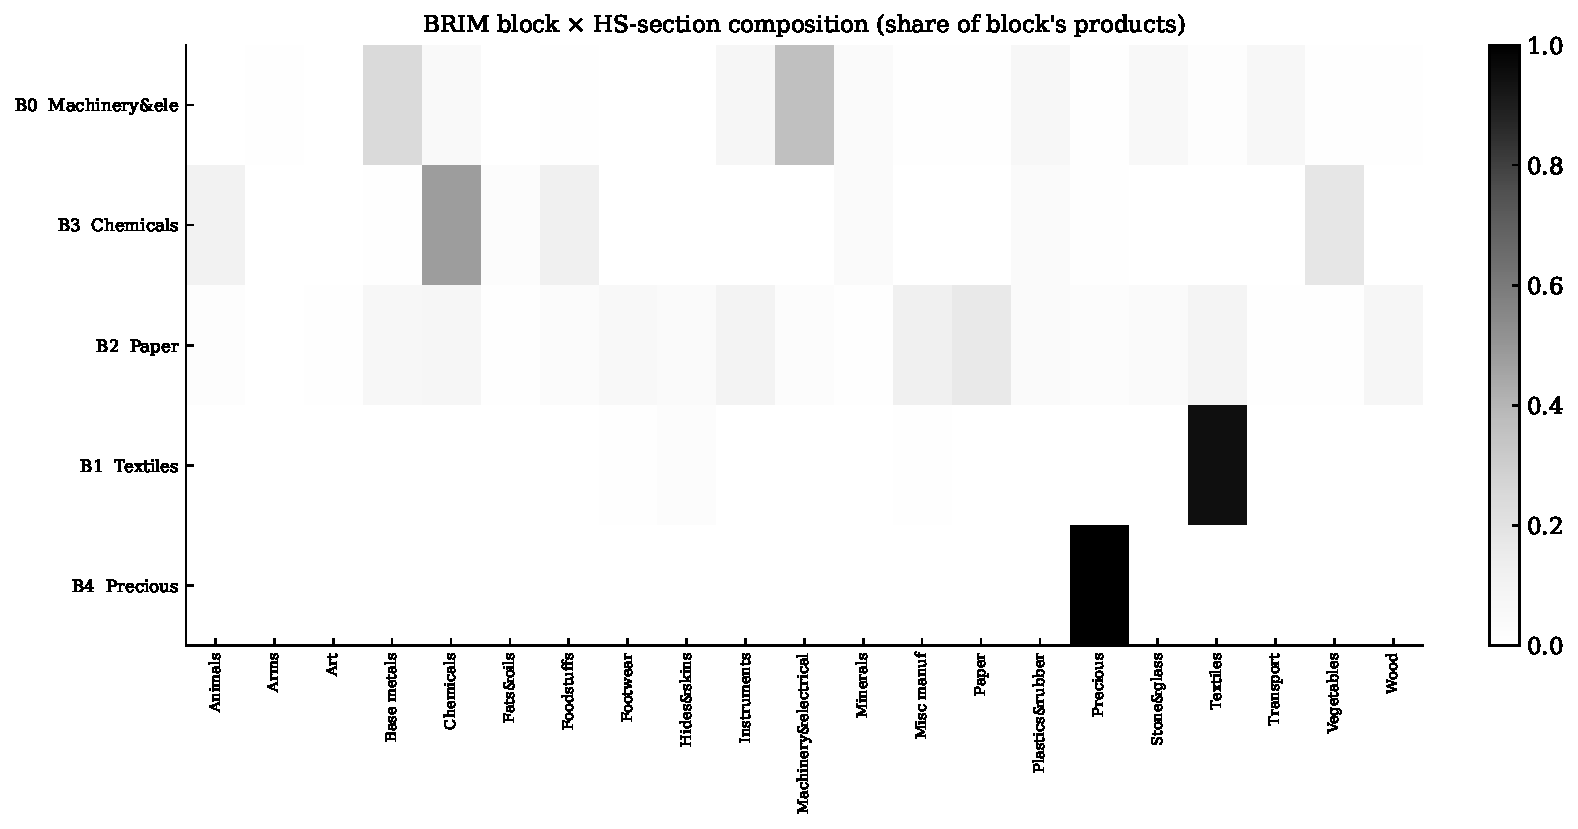
\includegraphics[width=0.93\textwidth]{ds_fig2_block_sections.pdf}
\caption{Capability block $\times$ HS-section composition. Textiles (B1) is near-pure;
the generalist block (B0) spreads across machinery, metals and instruments. The off-%
diagonal mass is the evidence that blocks are not industry codes.}
\label{fig:blocksec}
\end{figure}

\paragraph{Does the resolution matter? ($\gamma=1$ vs $\gamma=2$).} The block \emph{count}
is not an invariant --- it depends on $\gamma$. To check that the substantive findings do
not hinge on it, I re-ran the entire pipeline at the finer $\gamma=2$, which penalises the
null more and so returns more, smaller blocks (Table~\ref{tab:gamma},
Fig.~\ref{fig:g2sec}). Some of the split is \emph{economically meaningful}: agri-food,
bundled with chemicals at $\gamma=1$, separates into its own block, and dedicated footwear
and transport blocks emerge. Some is \emph{mechanical}: the pure textile block splits into
two near-identical sub-blocks, while the machinery--metals generalist stays mixed at any
resolution (it is where the bulk of firms sit). The point is that the \emph{conclusions are
invariant and only the levels rescale}: the structure is strongly modular and not a
relabelling of HS sectors at both resolutions, and out-of-block exploration tracks
destination reach rather than export value at both. What does move is the in/out
accounting --- finer blocks mean smaller in-block menus, so the out-of-block share
mechanically rises (pure-in-block $54.5\%\!\to\!43.2\%$). The lesson I carry to the panel:
\emph{fix one partition choice and read $\dout$ within a resolution, never across.}

\begin{table}[H]\centering\small
\caption{The same pipeline at two resolutions. Levels rescale; conclusions do not.}
\label{tab:gamma}
\begin{tabular}{@{}lcc@{}}
\toprule
Quantity & $\gamma=1$ (baseline) & $\gamma=2$ \\
\midrule
BRIM blocks                              & 5      & 10     \\
Bipartite modularity $\QB$               & 0.505  & 0.544  \\
ARI vs HS sections                       & 0.29   & 0.32   \\
HS sections spanned per block (avg)      & 13     & 9.4    \\
Pure in-block ($\sharecore=1$)           & 54.5\% & 43.2\% \\
$\mathrm{corr}(\dout,\text{dest.\ reach})$ & 0.18   & 0.16   \\
$\mathrm{corr}(\dout,\text{export value})$ & 0.03   & 0.06   \\
\bottomrule
\end{tabular}
\end{table}

\begin{figure}[H]\centering
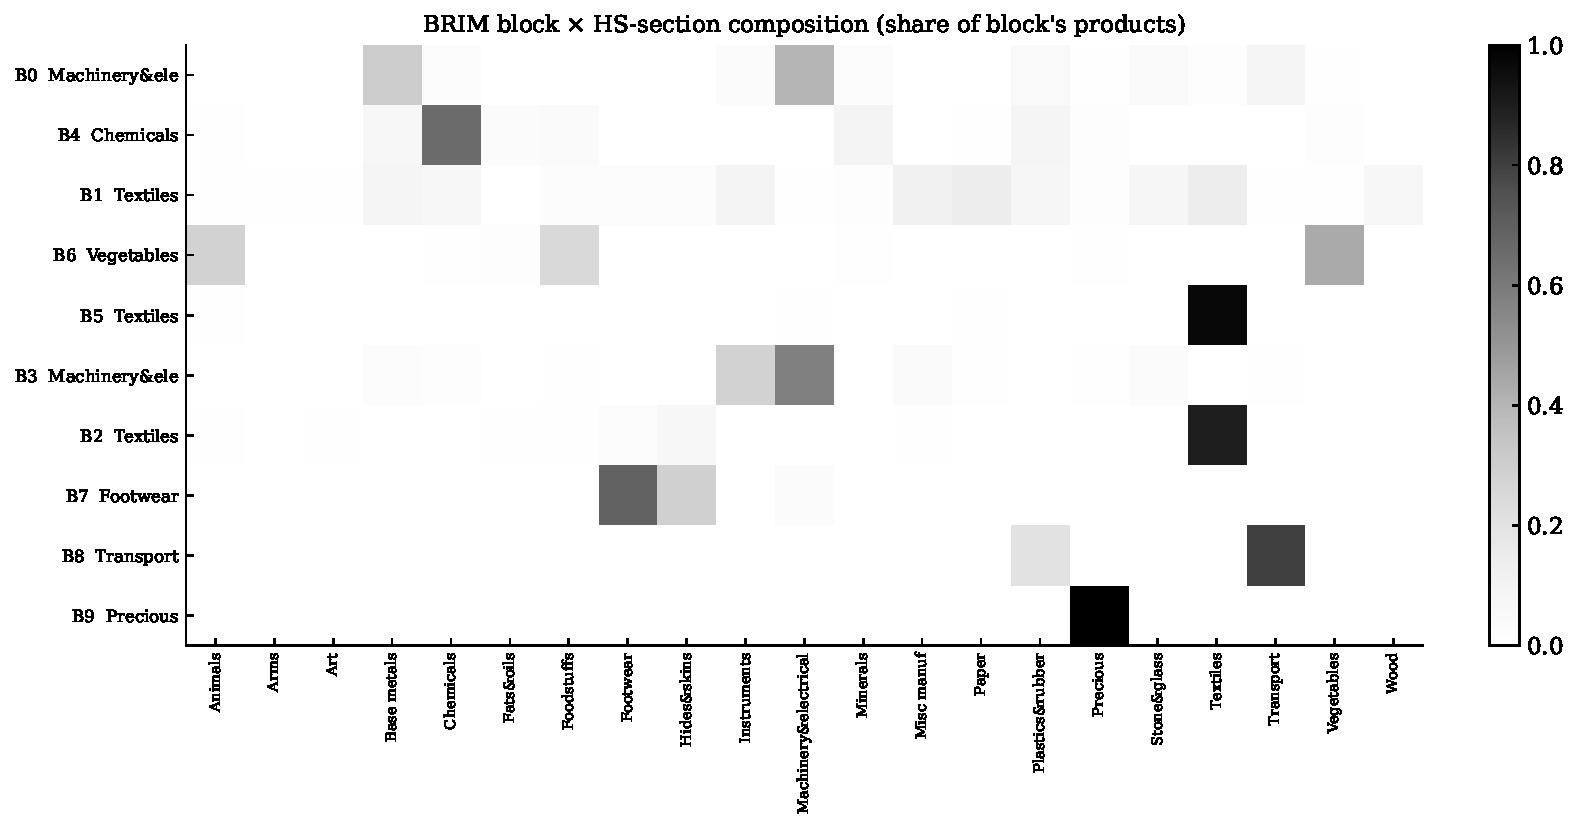
\includegraphics[width=0.90\textwidth]{ds_g2_block_sections.pdf}
\caption{$\gamma=2$: the ten finer blocks $\times$ HS sections (compare with the five-block
$\gamma=1$ map, Fig.~\ref{fig:blocksec}). The newly isolated dark cells --- a second
textile block, a separated chemicals block, footwear, transport, precious --- are the
meaningful splits; the machinery generalist (and the light-manufacturing catch-all) stay
spread, because they are genuinely entangled at any resolution.}
\label{fig:g2sec}
\end{figure}

\paragraph{These exporters are exploitation-heavy.} Splitting diversification into
$\din$ (competitive products \emph{inside} the firm's own block) and $\dout$ (those
\emph{outside} it), the picture is one of deep specialisation (Table~\ref{tab:div},
Fig.~\ref{fig:div}): mean $\din=13.0$ against mean $\dout=2.5$, and the out-of-block
margin is \emph{exactly zero for 54.5\% of firms}. The concentration index
$\sharecore=\din/(\din+\dout)$ has a median of $1.0$ and a large mass at the ceiling.
In March's language, the established Chinese exporter grows along the $\din$ axis,
within its capability block. \textbf{That distributional fact is what most shapes the
panel design}: $\dout$ is zero-inflated and floor/ceiling-bound,
so the ``reinvention'' falsifier ($\dout\!\uparrow$) is better-powered than the
``retrenchment'' direction, and the outcome models have to respect the count/zero-mass
structure (see \S\ref{sec:panel}).

\begin{table}[H]\centering\small
\caption{Diversification indicators ($N=71{,}017$). $\dout=0$ for the majority.}
\label{tab:div}
\begin{tabular}{@{}lrrrrrrr@{}}
\toprule
 & mean & sd & p10 & p25 & median & p75 & p90 \\
\midrule
$\din$            & 13.01 & 20.83 & 2 & 4 & 7 & 14 & 29 \\
$\dout$           &  2.53 & 11.38 & 0 & 0 & 0 &  2 &  5 \\
$\sharecore$      & 0.888 & 0.162 & 0.63 & 0.80 & 1.00 & 1.00 & 1.00 \\
\bottomrule
\end{tabular}

\smallskip
\footnotesize Pure in-block ($\sharecore=1$): 54.5\%. Mixed: 45.5\%. Pure out-of-block: 0\%.
\end{table}

\begin{figure}[H]\centering
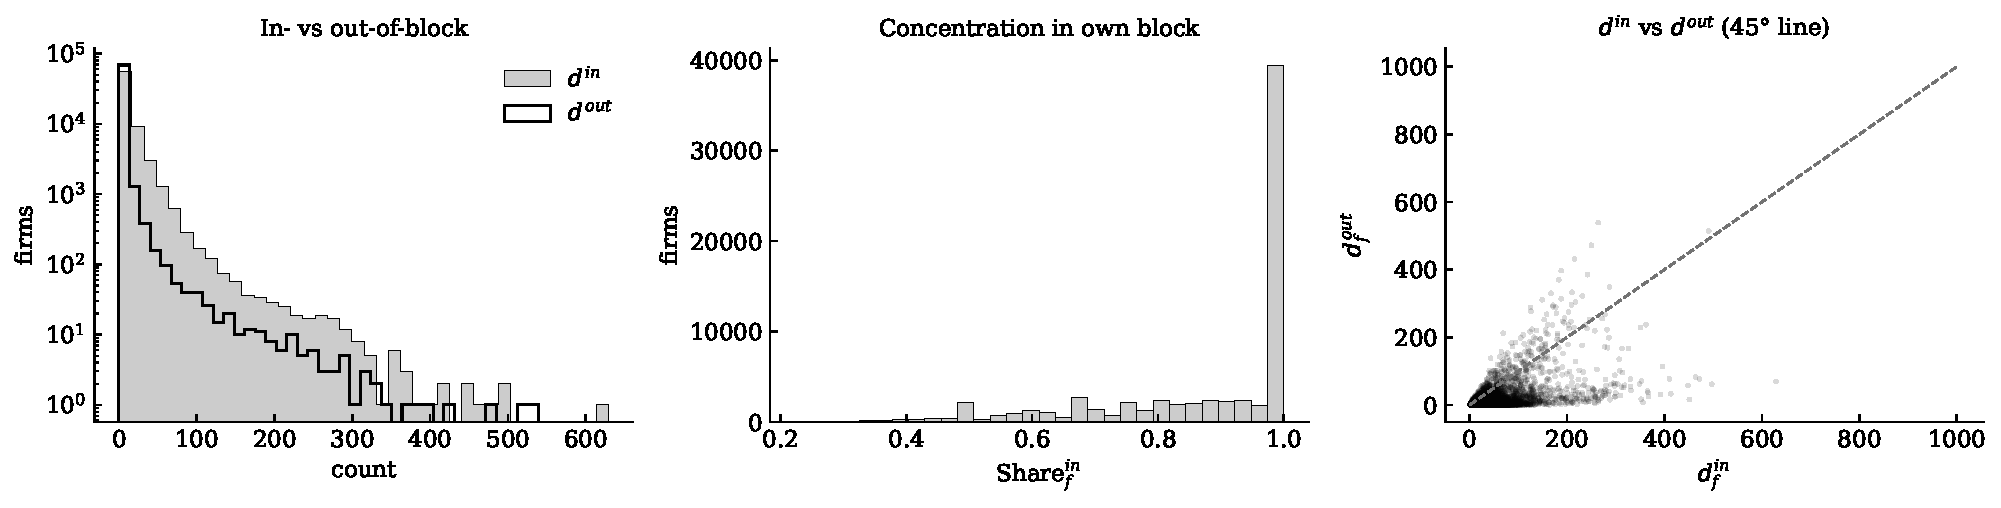
\includegraphics[width=0.99\textwidth]{ds_fig3_diversification.pdf}
\caption{\textbf{Left:} $\din$ vs $\dout$ (log $y$); $\din$ dominates, $\dout=0$ for the
median firm. \textbf{Centre:} $\sharecore$, with a mass at $1$ (pure specialists).
\textbf{Right:} $\din$ vs $\dout$ with the $45^\circ$ line --- the cloud lies below it,
firms grow within their block.}
\label{fig:div}
\end{figure}

\paragraph{A second pattern: out-of-block exploration is a \emph{geographic} signature, not
a size one.} Because the microdata carry the destination, I can give $\dout$ an economic
identity. Across $71{,}017$ firms, $\dout$ correlates with \emph{destination reach}
(number of countries served) at $0.18$, but with \emph{export value} at only $0.03$
(Spearman). Reaching more markets tracks out-of-block exploration; sheer revenue does
not (Fig.~\ref{fig:dest}). Holding destination reach fixed, scaling up in value actually
\emph{lowers} the out-of-block share (it deepens the core): a clean monotone pattern
at the baseline resolution, though the one finding that partially reverses under a finer
partition, so I read it cautiously. The message that survives: \textbf{the ``explorer''
firm is the wide-reach exporter, not the big-revenue one}, and exploration is concentrated in
particular blocks (the paper/light-manufacturing block explores three times as much as
any other). That is what tells me the eventual design must track the product and the
geographic margins \emph{jointly}, and must guard against export intermediaries, whose
unrelated baskets produce spuriously high $\dout$ and low portfolio coherence.

\begin{figure}[H]\centering
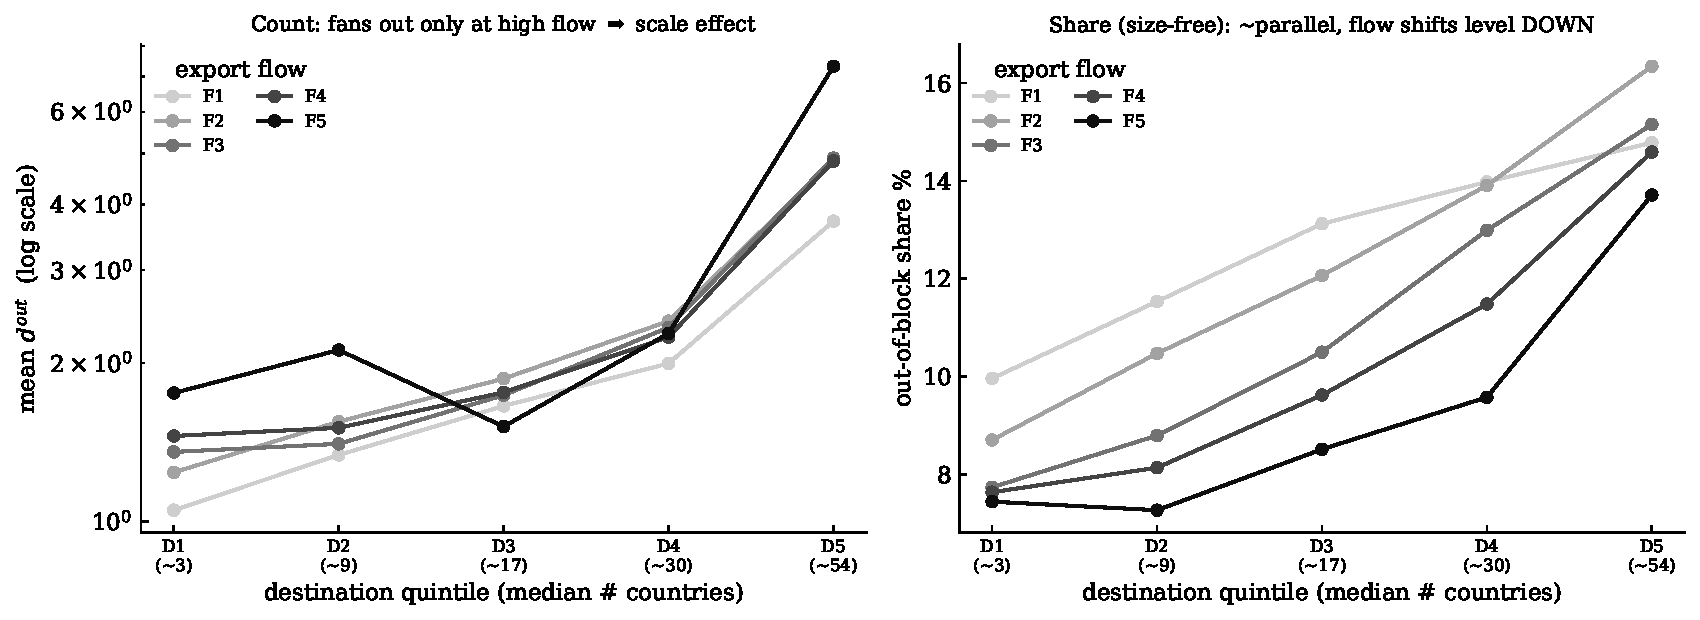
\includegraphics[width=0.99\textwidth]{ds_fig6_dest_interaction.pdf}
\caption{Out-of-block exploration by export-flow quintile (light $=$ low to dark $=$ high)
$\times$ destination reach. \textbf{Left:} mean $\dout$ count (log) --- rises with
destinations. \textbf{Right:} size-free out-of-block share --- again rises with
destinations, with the high-flow lines sitting \emph{below}. Breadth tilts the portfolio
outward; volume pulls it inward.}
\label{fig:dest}
\end{figure}

% =============================================================================
\section{From description to causation: the problem, and where I need your intuition}
\label{sec:panel}
% =============================================================================

The static layer is descriptive. The causal question (does an adverse trade shock push
the firm toward $\din$ or $\dout$?) needs a firm-by-year panel of the outcomes and a
credibly exogenous shock. Two of the three moving parts I think are tractable; the third
is genuinely open, and it is where I would most value your intuition. I lay out the
problem and my candidate fixes, and then ask what \emph{you} would do.

\paragraph{The shock --- I think this part is in hand.} I plan a continuous Bartik tariff
dose
\[
  \mathrm{TariffShock}_{it}=\sum_p \underbrace{s_{ip,\mathrm{pre}}}_{\text{pre-shock shares}}
  \cdot\underbrace{\varepsilon_p}_{\text{Fontagn\'e et al.\ 2022}}
  \cdot\underbrace{\Delta\ln(1+\tau_{pt})}_{\text{Teti GTD 2024}},
\]
estimated through a distributed-lag event study (leads $=$ parallel-trends test, lags $=$
hysteresis) with Ad\~ao et al.\ (2019) shift-share-robust standard errors. The exposure
shares are pre-shock and the elasticities $\varepsilon_p$ are external product parameters
estimated on the world trade matrix, so they cannot be a function of the Chinese firms I
study --- this side of the design is predetermined by construction. I keep the dose
\emph{continuous} on purpose: discretising into treated/control throws away the
exposure-intensity variation that identifies the dose--response (the cost is a stronger
parallel-trends requirement, which I can probe but not fully test).

\paragraph{The hard part --- turning a static map into a panel.} Here is the crux, and the
reason I want the algorithm understood (\S\ref{sec:china}). The capability blocks are
estimated on the \emph{pooled} network. A panel needs the outcome to vary over time, but
$\din/\dout$ are defined \emph{relative to the partition}, so the instant the partition
itself moves, the outcome and its own measuring instrument move together. There are two
routes, each with a cost:
\begin{itemize}[leftmargin=1.5em]
  \item \textbf{(a) Re-estimate the partition every year.} Conceptually attractive
        (capabilities really do evolve), but it makes block membership co-move with the
        shock: a tariff that pushes a firm off a product can show up as the \emph{product}
        switching blocks, so the treatment is absorbed \emph{into} the measuring instrument
        instead of being read \emph{against} it. Worse, the temporal-coupled multilayer
        machinery (Mucha et al.\ 2010) one would use to smooth the yearly slices
        \emph{couples adjacent years}, so the block at $t$ depends on $t{+}1$: a
        look-ahead that disqualifies it as a clean right-hand-side panel object. (It is
        also computationally heavy: BRIM on each yearly slice at the full $\sim$460k-firm
        scale.)
  \item \textbf{(b) Estimate the partition once on pre-shock years and hold it fixed,}
        letting only the firm's RCA incidence vary. This keeps the measuring instrument
        exogenous to the shock, at the cost of a map that grows stale --- classical
        measurement error, which attenuates \emph{toward} zero. That is an honest bias, not
        a confound, but it is a real loss of power.
\end{itemize}

\noindent My current lean is (b) as the baseline, with a \emph{pre-shock-evolving} map
(estimated only on pre-shock slices) as robustness, and --- the option I am most drawn to
but least sure of --- a binary, staggered design whose \emph{not-yet-treated} firms
could anchor a partition that evolves \emph{contemporaneously yet stays exogenous}, in the
spirit of a clean control group. \textbf{This single choice is the thing I would most like
your view on:} is the cleaner estimand worth a held-fixed (and therefore stale) map, or is
there a smarter way to let the capability geometry move \emph{with} the data without
letting it move \emph{with the treatment}?

\paragraph{What the preliminary data already dictate (whatever I decide above).} The static
layer is not just motivation; it pins down choices. (i)~$\din$ is the cleanest outcome;
$\dout$ is $54.5\%$ zeros $\Rightarrow$ a count/PPML model, not OLS. (ii)~The ceiling at
$\sharecore=1$ means the retrenchment direction is poorly powered and the
$\dout\!\uparrow$ falsifier is the sharper test. (iii)~Effects should vary by destination
reach and by block, since that is where exploration lives. (iv)~Coherence flags
intermediaries (unrelated baskets, spurious $\dout$) and must be a control. (v)~The
balanced core is economically dominant but selected --- external validity to the
entry/exit tail is a stated caveat, and it interacts with the exit problem below.

% =============================================================================
\section{Open issues, and the questions I would like your view on}
\label{sec:questions}
% =============================================================================

I separate what I already see as the \emph{soft spots} from the \emph{questions} I would
genuinely like to put to you. I have grouped the questions by mechanism, by empirical
design, and by theory, but the most valuable feedback would be on which of these is the
binding constraint on the project.

\subsection*{Soft spots I am already worried about}
\begin{enumerate}[leftmargin=1.5em]
  \item \textbf{The within-China RCA denominator under an aggregate shock.} Blocks are
        built from the Chinese firm--product network, so a China-relative Balassa is the
        internally consistent benchmark --- but a sector-wide tariff shock moves the
        aggregate Chinese export of a treated product for \emph{all} exposed firms,
        mechanically shifting threshold crossings. I treat this as an inference issue
        (leave-one-out and ex-China BACI denominators as robustness), but it is really a
        \emph{general-equilibrium} contamination of my own measure.
  \item \textbf{Exit selection.} The shock induces exit (Crozet et al.\ 2021); exited
        firms have no $\din/\dout$, so survivors are selected. I plan an exit equation
        plus Lee/IPW bounds and read the headline as conservative --- but the balanced-%
        sample design already conditions on survival, which may understate the very
        margin I care about.
  \item \textbf{Spillovers / SUTVA.} A tariff on one product reallocates demand to
        substitutes held by \emph{other} firms in the same block; Adao et al.\ (2019)
        absorbs the correlation in the SE but not the causal interference.
  \item \textbf{Zero-inflation and power.} With $\dout=0$ for the majority, the
        retrenchment direction may be statistically hard to move; the design may end up
        better at \emph{rejecting} reinvention than \emph{confirming} retrenchment.
\end{enumerate}

\subsection*{(A) Questions on the mechanism}
\begin{enumerate}[leftmargin=1.5em]
  \item Is retrenchment to the core best read as \emph{defensive pruning} (shedding the
        cheapest-to-cut peripheral products) or \emph{active consolidation} (reinvesting
        in the core)? These have the same $\sharecore$ signature but opposite welfare
        readings. Is there a margin in the data --- e.g.\ the complexity of the products
        \emph{dropped} (Nomaler--Verspagen 2023) --- that can separate them?
  \item The destination finding suggests $\dout$ is partly a \emph{geographic} object.
        Should the unit of analysis be the firm--product matrix (following the
        capability-network tradition) or a firm--product--destination tensor? Does
        promoting to the tensor buy identification, or just noise?
  \item Is ``exploration'' through $\dout$ genuinely capability-building, or is a large
        share of it intermediary churn that coherence controls cannot fully remove?
\end{enumerate}

\subsection*{(B) Questions on the empirical design / how to innovate the analysis}
\begin{enumerate}[leftmargin=1.5em]
  \item \textbf{The held-fixed-vs-evolving map trade-off} (the open seam of
        \S\ref{sec:panel}). Beyond the two routes I sketched, is there a third I am
        missing --- for instance a \emph{partition-free} outcome (a continuous relatedness
        or coherence score of the basket) that would sidestep the timing problem
        altogether, at the cost of losing the crisp in/out split? Which would you reach
        for?
  \item \textbf{Parallel trends for a continuous dose.} Beyond plotting lead
        coefficients, what is the most convincing way to defend ``no selection into dose
        level'' when the dose is a smooth shift-share and there is no clean control group?
  \item \textbf{The denominator problem.} Is the within-China RCA benchmark defensible
        under an aggregate shock, or should I move to an ex-China (rest-of-world) benchmark
        as the headline and pay the cost of a less internally consistent block definition?
  \item Given the zero-inflation, is there a better-powered \emph{single} outcome (a
        product-level retention hazard, in the spirit of Fontagn\'e et al.\ 2018) than
        the firm-level $\sharecore$?
\end{enumerate}

\subsection*{(C) A theoretical model --- here I am more interested in what occurs to you}
On the theory side I have instincts but no commitment, and this is where your reaction
matters most --- so these are deliberately open.
\begin{enumerate}[leftmargin=1.5em]
  \item If you wanted to rationalise an in-block/out-of-block margin, \emph{what backbone
        would you reach for}? My own instinct drifts toward a multi-product firm with a
        product ladder ranked by distance from a core capability (the ``core competence''
        tradition), where a tariff shock tilts the relative profitability of in- vs
        out-of-block products --- but I suspect there are cleaner objects, and I would
        rather hear what comes to mind than defend mine.
  \item Is there a natural way to make the \emph{sign} endogenous --- retrenchment for
        most firms, reinvention for a high-capability tail --- as a comparative static in a
        single state variable (capability stock, or distance-to-core)? That is the form in
        which March's (1991) verbal tension would become testable, but I do not yet see the
        minimal model that gives it.
  \item Does any of this \emph{need} general equilibrium? The within-China RCA denominator
        is itself a GE object, so the aggregate-shock ``contamination'' of my measure
        (soft spot 1) might be better treated as a structural feature inside a quantitative
        trade model --- which would also let me speak to the \emph{welfare} of retrenchment,
        not just its sign. Is that worth the modelling cost, or a distraction from a clean
        reduced-form paper?
  \item If you did build it, which empirical moment would you discipline it on first --- the
        dose--response slope, the $\din/\dout$ heterogeneity by strategic dependence, or the
        destination-reach gradient?
\end{enumerate}

\bigskip
\begin{keybox}
\noindent\textbf{What I would most like to leave the meeting with.}\ A judgement on the
binding constraint: is this project limited by \emph{identification} (the map-timing
choice and the continuous dose), by \emph{measurement} (the RCA denominator and
intermediaries), or
by the absence of a \emph{theoretical} object that makes the $\din/\dout$ split a
structural quantity? My current bet is that the empirics can carry a first paper on their
own, with the model as a second-stage companion --- but I would like to pressure-test
that ordering with you.
\end{keybox}

% =============================================================================
\appendix
\section{Supporting figure: heavy-tailed structure}
% =============================================================================
\begin{figure}[H]\centering
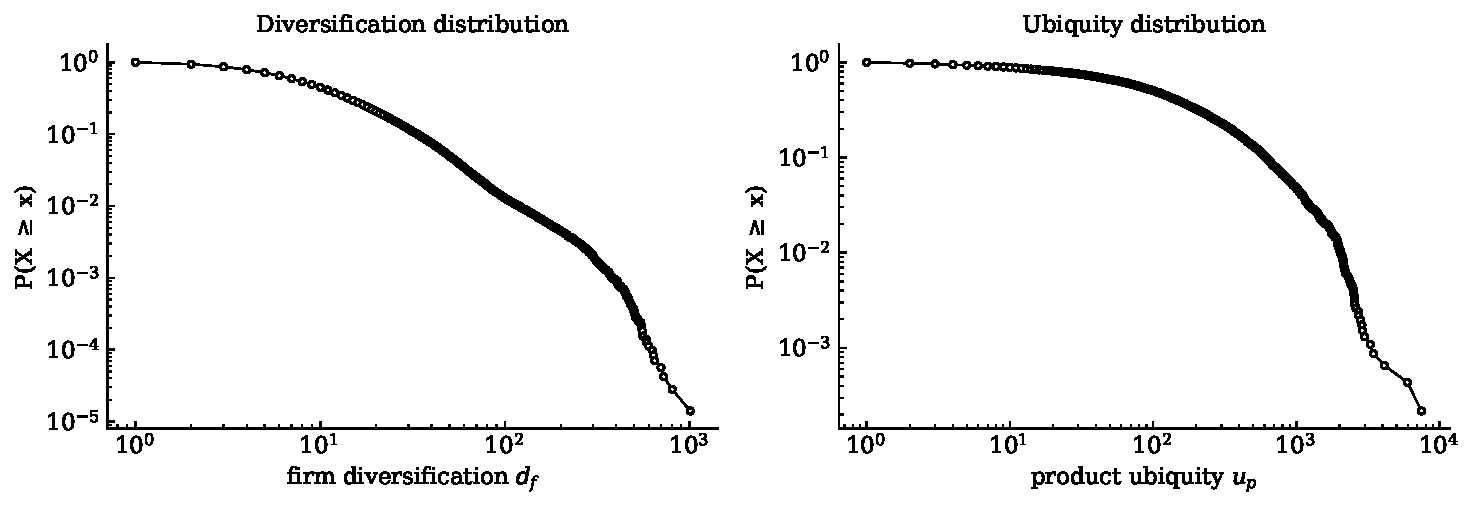
\includegraphics[width=0.88\textwidth]{ds_fig1_distributions.pdf}
\caption{Complementary CDFs of firm diversification $d_f$ (left) and product ubiquity
$u_p$ (right), log--log axes. Most firms are specialised and a few hugely diversified;
most products niche and a few near-universal --- the standard economic-complexity
signature, which the block structure then organises.}
\label{fig:dist}
\end{figure}

% =============================================================================
\section*{Selected references}
\addcontentsline{toc}{section}{Selected references}
\footnotesize
\begin{itemize}[leftmargin=1.4em,labelsep=0.4em]\raggedright
  \item Ad\~ao, R., Koles\'ar, M., Morales, E. (2019). Shift-share designs: theory and inference. \emph{Quarterly Journal of Economics} 134(4): 1949--2010.
  \item Aghion, P., Bloom, N., Blundell, R., Griffith, R., Howitt, P. (2005). Competition and innovation: an inverted-U relationship. \emph{Quarterly Journal of Economics} 120(2): 701--728.
  \item Akcigit, U., Melitz, M. (2022). International trade and innovation. \emph{Handbook of International Economics}, vol.~5.
  \item Amiti, M., Konings, J. (2007). Trade liberalization, intermediate inputs, and productivity: evidence from Indonesia. \emph{American Economic Review} 97(5): 1611--1638.
  \item Arjona, R., Connell, W., Herghelegiu, C. (2023). An enhanced methodology to monitor the EU's strategic dependencies and vulnerabilities. European Commission, DG GROW Working Paper.
  \item Barber, M. J. (2007). Modularity and community detection in bipartite networks. \emph{Physical Review E} 76(6): 066102.
  \item Bernardo, A. E., Chowdhry, B. (2002). Resources, real options, and corporate strategy. \emph{Journal of Financial Economics} 63(2): 211--234.
  \item Bottazzi, G., Secchi, A. (2006). Gibrat's law and diversification. \emph{Industrial and Corporate Change} 15(5): 847--875.
  \item Bruno, M., Mazzilli, D., Patelli, A., Squartini, T., Saracco, F. (2023). Inferring comparative advantage via entropy maximization. \emph{Journal of Physics: Complexity} 4: 045011.
  \item Callaway, B., Goodman-Bacon, A., Sant'Anna, P. H. C. (2024). Difference-in-differences with a continuous treatment. NBER Working Paper 32117.
  \item Crozet, M., Hinz, J., Stammann, A., Wanner, J. (2021). Worth the pain? Firms' exporting behaviour to countries under sanctions. \emph{European Economic Review} 134: 103683.
  \item Crozet, M., Fernandes, A. M., Mayer, T., Milet, E., Taglioni, D. (2025). Phyloeconomic trade diversity: the impact of diversification on firms' export volatility for 64 developing countries. Working Paper.
  \item De Stefano, V., Mula, M., Mariani, M. S., Zaccaria, A. (2025). From macro to micro: economic complexity indicators for firm growth. arXiv:2507.21754.
  \item Farrell, H., Newman, A. L. (2019). Weaponized interdependence: how global economic networks shape state coercion. \emph{International Security} 44(1): 42--79.
  \item Fontagn\'e, L., Secchi, A., Tomasi, C. (2018). Exporters' product vectors across markets. \emph{European Economic Review} 110: 150--180.
  \item Fontagn\'e, L., Guimbard, H., Orefice, G. (2022). Tariff-based product-level trade elasticities. \emph{Journal of International Economics} 137: 103593.
  \item Hidalgo, C. A., Hausmann, R. (2009). The building blocks of economic complexity. \emph{PNAS} 106(26): 10570--10575.
  \item Korniyenko, Y., Pinat, M., Dew, B. (2017). Assessing the fragility of global trade: the impact of localized supply shocks using network analysis. IMF Working Paper 17/30.
  \item Le, N. A., Tomasi, C. (2023). Trade liberalization and firms' productivity in Vietnam: the role of local business environment. \emph{Regional Studies} 57(9): 1681--1713.
  \item March, J. G. (1991). Exploration and exploitation in organizational learning. \emph{Organization Science} 2(1): 71--87.
  \item Matsusaka, J. G. (2001). Corporate diversification, value maximization, and organizational capabilities. \emph{Journal of Business} 74(3): 409--431.
  \item Mucha, P. J., Richardson, T., Macon, K., Porter, M. A., Onnela, J.-P. (2010). Community structure in time-dependent, multiscale, and multiplex networks. \emph{Science} 328(5980): 876--878.
  \item Nomaler, \"O., Verspagen, B. (2023). Related or unrelated diversification: what is smart specialization? UNU-MERIT Working Paper.
  \item Pavcnik, N. (2002). Trade liberalization, exit, and productivity improvements: evidence from Chilean plants. \emph{Review of Economic Studies} 69(1): 245--276.
  \item Penrose, E. T. (1959). \emph{The Theory of the Growth of the Firm}. Basil Blackwell, Oxford.
  \item Pugliese, E., Napolitano, L., Zaccaria, A., Pietronero, L. (2019). Coherent diversification in corporate technological portfolios. \emph{PLOS ONE} 14(10): e0223403.
  \item Tacchella, A., Cristelli, M., Caldarelli, G., Gabrielli, A., Pietronero, L. (2012). A new metrics for countries' fitness and products' complexity. \emph{Scientific Reports} 2: 723.
  \item Teece, D. J. (1982). Towards an economic theory of the multiproduct firm. \emph{Journal of Economic Behavior \& Organization} 3(1): 39--63.
  \item Teti, F. (2024). The Global Tariff Database: 30 years of trade policy. CESifo Working Paper 11590.
  \item Topalova, P. (2010). Factor immobility and regional impacts of trade liberalization: evidence on poverty from India. \emph{American Economic Journal: Applied Economics} 2(4): 1--41.
  \item Valvano, S., Vannoni, D. (2003). Diversification strategies and corporate coherence: evidence from Italian leading firms. \emph{Review of Industrial Organization} 23: 25--41.
  \item Vannoorenberghe, G., Wang, Z., Yu, Z. (2016). Volatility and diversification of exports: firm-level theory and evidence. \emph{European Economic Review} 89: 216--247.
\end{itemize}

\end{document}
